\section{Ground Heat Transfer Calculations using C and F Factor Constructions}\label{ground-heat-transfer-calculations-using-c-and-f-factor-constructions}

Building energy code and standards like ASHRAE 90.1, 90.2 and California Title 24 require the underground wall constructions and slabs-on-grade or underground floors not to exceed certain maximum values of C-factor and F-factor, which do not specify detailed layer-by-layer materials for the constructions. If using the normal approach (layer by layer) of ground constructions with EnergyPlus, users would need to create a pseudo wall or floor construction to match the thermal performance such as thermal mass effect and U-factor, and rely on the EnergyPlus Basement and Slabs tools to generate the monthly ground temperatures.

A simplified approach is introduced to create equivalent constructions and model the ground heat transfer through underground walls and ground floors for the building energy code compliance calculations. The approach is to create constructions based on the user defined C or F factor with two layers: one concrete layer (0.15 m thick) with thermal mass, and one fictitious insulation layer with no thermal mass.

Three objects are used in the C and F factor calculations:

\begin{itemize}
\item
  Construction:CfactorUndergroundWall
\item
  Construction:FfactorGroundFloor
\item
  Site:GroundTemperature:FCfactorMethod
\end{itemize}

Site:GroundTemperature:FCfactorMethod is used only by the underground walls or slabs-on-grade or underground floors defined with C-factor (Construction:CfactorUndergroundWall) and F-factor (Construction:FfactorGroundFloor) method for code compliance calculations where detailed construction layers are unknown. Only one such ground temperature object can be included. The monthly ground temperatures for this object are close to the monthly outside air temperatures delayed by three months. If user does not input this object in the IDF file, it will be defaulted to the 0.5m set of monthly ground temperatures from the weather file if they are available.

Detailed description of the three objects is in the Input Output Reference document. The following section describes how the equivalent material layers are created based on the C-factor and F-factor.

\subsubsection{Slab-on-grade and Underground Floors Defined with F-factors}\label{slab-on-grade-and-underground-floors-defined-with-f-factors}

The steady state heat transfer through the floor is calculated as,

\begin{equation}
  Q = \text{Area} \cdot U_{eff} \cdot (T_{air,out} - T_{air,in}) = (T_{air,out} - T_{air,in}) \cdot (P_{exp} \cdot \text{F-factor})
\end{equation}

Where,

\(Q\) is the steady state heat transfer through the floor in Watt

Area is the area of the floor in m\(^{2}\)

\(U_{eff}\) is the effective heat transfer coefficient including the floor construction, the soil, and the thermal resistance of the interior and exterior air films.

\(T_{air,in}\) is the indoor air temperature in °C

\(T_{air,out}\) is the outside air temperature in °C

\(P_{exp}\) is the exposed perimeter of the floor in m

F-Factor is the heat transfer through the floor, induced by a unit temperature difference between the outside and inside air temperature, on the per linear length of the exposed perimeter of the floor. The unit is W/m·K.

Therefore,

\begin{equation}
U_{eff} = (P_{exp} \cdot \text{F-factor}) / Area
\end{equation}

\begin{equation}
1 / U_{eff} = R_{eff} + R_{film,in} + R_{film,out}
\end{equation}

\begin{equation}
R_{eff} = Area / (P_{exp} \cdot \text{F-factor}) - R_{film,in} - R_{film,out}
\end{equation}

Where,

R\(_{eff}\) is the effective thermal resistance in m\(^{2}\)·K/W, including the soil and the floor construction

R\(_{film,in}\) and R\(_{film,out}\) are the air film resistance of the inside and outside surfaces, respectively.

The outside air film resistance R\(_{film,out}\) = 0.03 m\(^{2}\)·K/W. The inside air film resistance R\(_{film,in}\) = 0.135 m\(^{2}\)·K/W, which is the average of the 0.16 m\(^{2}\)·K/W for heat flow down and 0.11 m\(^{2}\)·K/W for heat flow up.

Approximate the thermal mass of the floor construction with a 6-inch (0.15 m) heavy concrete, and use a fictitious insulation layer with no thermal mass to match the thermal resistance of the construction.

We have,

\begin{equation}
R_{fic} = R_{eff} - R_{con}
\end{equation}

Where,

R\(_{fic}\) is the thermal resistance of the fictitious insulation layer in m\(^{2}\)·K/W.

R\(_{con}\) is the thermal resistance of the concrete layer in m\(^{2}\)·K/W.

Properties of the concrete layer are:

Thickness = 0.15 m

Conductivity = 1.95 W/m·K

Density = 2240 kg/m\(^{3}\)

Specific heat = 900 J/kg·K

R\(_{con}\) = 0.15/1.95 = 0.077 m\(^{2}\)·K/W

Finally,

\begin{equation}
R_{fic} = R_{eff} - 0.077
\end{equation}

\begin{figure}[hbtp] % fig 32
\centering

\includegraphics[width=0.9\textwidth, height=0.9\textheight, keepaspectratio=true]{media/image435.png}
\caption{Schematic for Slab on Grade - Two Spaces \protect \label{fig:schematic-for-slab-on-grade-two-spaces}}
\end{figure}

For slabs-on-grade as shown in the figure above, the exposed perimeter is (2A + C) for the Dining area, and (2B + C) for the Kitchen area. For underground floors with no exposed perimeter, the R\(_{eff}\) can be assumed a big value such as 1000 hr·ft\(^{2}\)·°F/Btu (177 m\(^{2}\)·K/W).

\textbf{\emph{Underground Walls Defined with C-Factors}}

The steady state heat transfer through the underground wall is calculated as,

\begin{equation}
Q = Area * U_{eff} * (T_{air,out} - T_{air,in})
\end{equation}

\begin{equation}
1 / U_{eff} = R_{eff} + R_{film,out} + R_{film,in}
\end{equation}

Where,

Q is the heat transfer through the wall in Watt

Area is the area of the wall in m2

U\(_{eff}\) is the effective heat transfer coefficient including the wall construction, the soil, and the thermal resistance of the interior and exterior air films.

R\(_{eff}\) is the effective thermal resistance in m\(^{2}\)·K/W, including the soil and the wall construction

R\(_{film,in}\) and R\(_{film,out}\) are the air film resistance of the inside and outside surfaces, respectively.

C-factor is the time rate of steady-state heat flow through unit area of the construction, induced by a unit temperature difference between the body surfaces. The C-Factor unit is W/m\(^{2}\)·K. The C-factor does not include soil or air films.

\begin{equation}
R_{eff} = 1/C-factor + R_{soil}
\end{equation}

R\(_{soil}\) is the effective R-value of the soil. Reference values from Table C6.10.1 of the SI version of the ASHRAE Standard 90.1-2010 are as follows:

\begin{figure}[htbp]
\centering
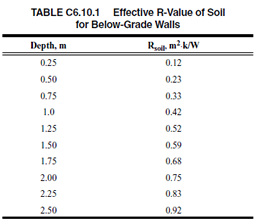
\includegraphics{media/image436.png}
\caption{Effective R-Value of Soil for Below-Grade Walls}
\end{figure}

A fairly good linear regression (R\(^{2}\) = 0.9967) for the above data is,

\begin{equation}
R_{soil} = 0.0607 + 0.3479 * Depth
\end{equation}

Approximate the thermal mass of the wall construction with a 6-inch (0.15 m) heavy concrete, and use a fictitious insulation layer with no thermal mass to match the thermal resistance of the construction. Then we have the thermal resistance of the insulation layer,

\begin{equation}
R_{fic} = R_{eff} - R_{con}
\end{equation}

Where,

R\(_{fic}\) is the thermal resistance of the fictitious insulation layer

R\(_{con}\) is the thermal resistance of the concrete layer in m\(^{2}\)·K/W.

Properties of the concrete layer are:

Thickness = 0.15 m

Conductivity = 1.95 W/m·K

Density = 2240 kg/m\(^{3}\)

Specific heat = 900 J/kg·K

R\(_{con}\) = 0.15/1.95 = 0.077 m\(^{2}\)·K/W
